%!TEX root = ../farid_msc_thesis.tex

\chapter{Related work}
\label{ch:related_work}

lalala

%
\subsection{Text mining}
%
Text mining (\textit{"knowledge discovery from textual databases"} \cite{tan1999text}) is the process and techniques used to extract relevant and non trivial information from unstructured text data.  In general, text data can be analyzed using lexical, sintactic or semantic approaches (for example, \textit{Part-of-Speech tagging}) or a vector space model). In order to extract meaningful information from text, they are usually represented according to their semantic rather than using string-based approaches ~\cite{aggarwal2012mining}.

Some fields related to text mining  involves information retrieval, text analysis, information extraction, clustering, categorization, visualization, database technology, machine learning and data mining ~\cite{tan1999text}.

%
\subsection{Empirical Laws in Linguistics}
%
There are some empirical laws in linguistics that try to explain some features of words in NLP context, specially in text documents.

Zipf's  law establishes an approximate mathematical relation between the frequency of occurrence of each word and its rank in the list of all words used in a text ordered by decreasing frequency ~\cite{montemurro2001beyond}.  The Zipf's law states the following relation:

\begin{center}
\begin{equation}
\label{ZipfLaw}
f(s)  \propto  \frac{A}{s^{\alpha}} 
\end{equation}
\end{center}


where \textit{{$\alpha$}} is slightly grater that 1, \textit{A} is a normalizing constant,  \textit{s} is an index of a given word, and \textit{f(s)} is the frequency of a word. This law can at most account for the statistical behavior of words frequencies in a limited zone (middle-low to low range of the rank variable) ~\cite{montemurro2001beyond}. \\

 Mandelbrot\'s law introduces a modification to the Zip's law, by using arguments on the fractal structure of lexical trees. The only improvement over the original Zip's law is that it fits better to regions corresponding to lowest ranks (s {$\le$} 100), dominated by function words ~\cite{montemurro2001beyond}: 

\begin{center}
\begin{equation}
\label{mandelbrotLaw}
f(s)  \propto  \frac{A}{(1+Cs)^{\alpha}} 
\end{equation}
\end{center}

where \textit(C) is a second parameter that needs to be adjusted to fit the data.\\

It has been argued that using these laws it is possible to discriminate between human writings and stochastic version of texts, just analyzing the statistical properties of words that fall beyond the scope where (Eq. \ref{mandelbrotLaw})  holds ~\cite{cohen1997numerical}.

Using these empirical laws, we can generate models in order to weight the importance of certain words, based on the frequency of words itself in a given text. Actually, \textit{stop-words} are considered with low relevance, because they have nothing semantically important about a document \cite{wilbur1992stopwords}.

%
\subsection{Word Embeddings}
%
Semantic word representation is based on the assumption that words with similar meanings are placed in similar contexts. 
In order to use a vector space model, it has been proposed  to represent words as dense vectors derived by training methods inspired in neural-network language modeling ~\cite{compositionality2013Mikolov}
. These kind of representations are referred to as \textit{"Neural Embeddings"} or \textit{"Word Embeddings"}. 

The main advantage of representing texts using word embeddings is that they are easy to work with (they are efficiently computational throw a low-dimensional matrix operations). On the other hand, word embeddings are considered opaque, in the sense that it is hard to assign meanings to the dimensions of the induced representation ~\cite{compositionality2013Mikolov}. 

\subsubsection{Skip-Gram Model}
The skip-gram neural model introduced by Mikolov et al. was trained using the negative-sampling procedure. 
In this model, each word \textit{$w \epsilon W$} is associated with a vector \textit{$v_w \epsilon R^d$} and similarly each context \textit{$c \epsilon C$} is represented as a vector \textit{$v_c \epsilon R^d$}, where \textit{W} are the words in vocabulary, \textit{C} is the context vocabulary, \textit{d} is the embedding dimensionality. The entries in vectors are latent, and treated as parameters to be learned. So, we are expecting parameters values such that the dot product between vectors \textit{$v_w \cdot v_c$} produce an  associated value, where a "good" word-context pair is maximized. 

The objective function in this algorithm can be summarized as:

\begin{center}
\begin{equation}
arg max_{v_w,v_c} (\sum_{(w,c)\epsilon D}log  \sigma(v_c \cdot v_w) + \sum_{(w,c)\epsilon D'}log \sigma(-v_c \cdot v_w))
\end{equation}
\end{center}

So, optimizing this objective function, where \textit{$\sigma(x) = 1/(1+e^x)$}, let us observe word-context pairs that have similar embeddings, while scattering unobserved pairs. Also, words that appear in similar context should have similar embeddings. 

An alternative of the Skip-Gram model proposed by \cite{compositionality2013Mikolov}, is to replace the bag-of-words (linear contexts) with arbitrary context ~\cite{levy2014dependency}.

%
\subsection{Compositional Distributional Semantics}
%

Semantics of words can be approximated by the patterns of co-occurrence of words in a corpus (statistical semantics as \textit{GloVe} proposes \cite{pennington2014GloVe}), or through formal semantics, where the idea of compositionality can be reached in terms of a syntax-driven calculus ~\cite{baroni2014frege}.

The term of \textit{Semantic compositionality} is about a complex expression, which is a function of the meaning of its constituent parts and how they are combined. For example, most of the  phrases in NLP are composed by a noun and a verb, or an adjective and a noun, such that when they are joined they acquire a special value. 

Mikolov et al. explored this approach in a multidimensional vector space where semantics of words are represented. He found that using neural networks to represent words, they encode linguistic regularities and patterns \cite{compositionality2013Mikolov}. He also found (using an empirical approach) that those patterns have a linear translation, in this way, using simple vector arithmetics on word vectors, some pattern preserve a linear structure. For example, word("Berlin")-word("Germany") + word("France") is closest to word("Paris"), using the cosine distance. 

\subsubsection{Composition by vector mixtures}
The most intuitive way of composing two word represented by vectors is by adding them (\textit{additive approach}) or multiplying them (\textit{multiplicative approach}).  The \textit{weighted additive model}, is when vectors are modified by a scalar value before summing them \cite{mitchell2010composition}, this approach works well in tasks of predicting human similarity judgments about adjective-noun, noun-noun, verb-noun and noun-verb phrases.

The components of additive vectors inherit the cumulative score mass from the input components. Multiplication, captures the interaction between the values in the input components. 
   

%
\subsection{Singular Value Decomposition (SVD)}
%
Singular Value Decomposition is a theorem from lineal algebra that says  that any m x n matrix  \textit{M} whose entries are real numbers, can be decomposed into three matrices (\textit{$U_{m,m}, S_{m,n}, V_{n,n}^{*}$}) , such that: 

\begin{center}
\begin{equation}
\label{SVD}
M  = U_{m,m}, S_{m,n}, V_{n,n}^{*}
\end{equation}
\end{center}

The matrix \textit{$V_{n,n}$} is diagonal, and its values in the main diagonal after applying the SVD are called \textit{singular values of M}, and they are ordered from greatest to least along the main diagonal of D. 

The singular values represent the "dimensions of meaning" for words and passages, when words are represented in a \textit{semantic vectorial space}. So, SVD is the base of the LSA (Latent Semantic Analysis) ~\cite{landauer1998introduction}, used for indexation and information retrieval. 

It is common to use the cosine distance (Eq. \ref{cosineDistance}) between words mapped into a vector space (\textit{A,B} are two vectors), in order to measure the similarity between them ~\cite{manningh}. 
one string into the other. 
\begin{center}
\begin{equation}
\label{cosineDistance}
cos (\theta ) =  \frac{\sum_{i=1}^{n} A_iB_i}{\sqrt{\sum_{i=1}^{n}{A_i}^{2}\sum }\sqrt{\sum_{i=1}^{n}B_i^{2}}}
\end{equation}
\end{center}

%
\subsection{Spelling correction of words}
Typos and misspelling words are commonly done when someone is filling out an application.  For this reason, an algorithm for correcting misspelling should be used, in order to acquire the complete semantic of a sentence without ignoring "inexistent" words that could be important. Otherwise, uncommon words (like those that are misspelled) should be discarded (according to Zipf's law, words with low frequency are not semantically important). 

Using Peter Norving's algorithm for spelling corrections let us discard some words from applications that seem to be meaningless, changing them for most appropriate words. In essence, this algorithm computes a set of \textit{similar} words, and proposes a candidate that maximizes the probability that this propose is the intended correction, given the original word. 
\begin{center}
\begin{equation}
\label{norving_bayes}
	argmax_{c \epsilon candidates} P(c|w)
\end{equation}
\end{center}

Using the Bayes's Theorem:
 
\begin{center}
\begin{equation}
\label{norving_bayes2}
	argmax_{c \epsilon candidates} P(c)P(w|c)
\end{equation}
\end{center}

In this case, the factor P(w) in the denominator was omitted, because it is the same for every possible candidate \textit(c).

The expression \ref{norving_bayes2} has four parts:
\begin{enumerate}  
\item Argmax.- It is used to select the best candidate, which is the one with highest probability computed. 
\item c $\epsilon$ candidates .- It indicates a candidate correction to consider from a set.
\item P(c) .- It can be seen as the language model. This indicates the probability that a word \textit{c} appears as a word in the language. 
\item P(w $\mid$ c).- This is the error model, which indicates the probability that \textit{w} would be typed in a text when it should meant \textit{c}. 
\end{enumerate}

The set of candidate words for this algorithm are computed using a \textit{Levenshtein Distance} of 1 and 2, and the proposed set of words are checked if they appear in the vocabulary of the language. 

\subsubsection{Levenshteing Distance}.
The Levenshtein distance (LD), also known as \textit{Edit distance}, is a measure of similarity between two strings. This distance is computed based on \textit{simple edition} to a word (it can be a \textbf{deletion},\textbf{transposition}, \textbf{replacement} or \textbf{insertion} ) required to transform one string into the other.

The set of words created using a Levenshteing distance of 1 is huge. For example, for a word of length \textit{n}, we have \textit{n} deletions, \textit{n - 1} transpositions, \textit{26n} alterations and \textit{26(n + 1) } insertions, giving a total of \textit{54n + 25} candidate words \cite{NorvingSpelling}. 
 

%

%
\subsection{Fuzzy Rule Based System}
%
Fuzzy logic emerged since 1965 \cite{Zadeh1965fuzzy}, and it is commonly used in many controlling processes, electronics devices, diagnosis systems and expert systems. This kind of logic is not restricted to zeros and ones (0,1) (it can be considered as an extension of multivalued logic). This kind of systems are useful when we want to make qualitative knowledge useful.

Usually, this qualitative knowledge is expressed in the form of rules like \textit{If(statement) then (conclusion)}, where the statement and the conclusion use \textit{linguistic variables}. These linguistic variables describe certain quantities from data, for example, 40 $^{\circ}$C can be transform into the linguistic value \textit{"hot"}.

In this case, the Fuzzy Rule Based System should approximate to a human being in a decision making process. In this way, the system has to take in to account the combination of observations and the weighing up between the inputs to the system. 

In order to express inputs and ouptus as linguistic forms, the Theory of Fuzzy Sets and Fuzzy Logic help. 

\subsubsection{Membership Functions}
 Membership functions works with linguistic variables. A linguistic variable is the one that express a quantity using linguistic values. For example, the linguistic variable "weight" has the linguistic value "heavy" for object with mass grater than 100 kg. 
 In this way, linguistic values are interpreted establishing \textit{membership functions} ($\mu_A(x)$). \\
 
 This functions can be seen as a curve with unsharp boundaries defined for all elements \textit{x} of the fundamental set \textit{X}. So, the input variables into the Fuzzy System are mapped to a membership value between 0 and 1 (\textit{degree of matching}). These ideas are similar to the theory of fuzzy sets \cite{zade1968}.

 \begin{center}
\begin{equation}
\label{fuzzySet}
	A = {(x, \mu_A(x)) | x \epsilon X }
\end{equation}
\end{center}

For example, the next diagram \cite{DIAGRAMA1} gives an example for linguistic value "high" of the linguistic variable "salary".

Using memberships functions, it is possible to indicate in which degree a linguistic statement is regarded as a fulfilled for a certain real value of the considered quantity.

\subsubsection{Fuzzy Operations}
Usually, Fuzzy Rules in Fuzzy Inference Systems are composed by two or more linguistic statements using operators like: \\


$\cdot$ \textbf{or}.- Maximum or algebraic sum (eg. temperature = high $\vee$ pressure = low).
\begin{center}
\begin{equation}
\label{fuzzySet11}
	\mu_C = max(\mu_A,\mu_B) 
\end{equation}

\begin{equation}
\label{fuzzySet12}
	\mu_C = \mu_A + \mu_B - \mu_A\bullet\mu_B
\end{equation}
\end{center}


$\cdot$ \textbf{and}.- Minimum or algebraic product (eg. temperature = low $\wedge$ humidity = high).
\begin{center}
\begin{equation}
\label{fuzzySet21}
	\mu_C = min(\mu_A, \mu_B) 
\end{equation}

\begin{equation}
\label{fuzzySet22}
	\mu_C = min(\mu_A, \mu_B) 
\end{equation}
\end{center}

$\cdot$ \textbf{not}.- Complement of a fuzzy set (eg. $\neg$ low = not(low)).
\begin{center}
\begin{equation}
\label{fuzzySet3}
	\bar{\mu_a} = 1 - \mu_a
\end{equation}
\end{center}
%

\subsection{Latent Dirichlet Allocations}
Description of the Latent Dirichlet Allocation (LDA) algorithm, 
that find \textit{n} topics in a document, and assigns a certain probability to each word to be part of a given topic. 

Once this algorithm was ``trained'', it is possible to make a query asking for ``proportions'' of probabilities that a query belongs to those \textit{n} topics.

\begin{figure}[h]
	\label{fig:lda_esquema}
	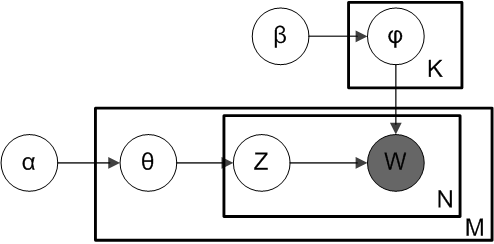
\includegraphics[width=\textwidth]{Smoothed_LDA.png}
    \caption{LDA diagram from wikipedia.}
\end{figure}

\subsection{Term Frequency- Inverse Document Frequency}
This form is used to proyect text data into a vectorial space. This algorithm use as input the well-known \textit{BagOfWords} (BOW) text representations, that builds a matrix where each row represent a document, and each column represent a word. In this way, a text corpus is represented as a matrix that captures the frecuency of each words of each document. 

Term -frequency establishes that most frequent words (terms \textit{t}) are the most important in a document \textit{d} (if a word is repeated many times, is because it should be important and relevant) (Eq. \ref{tf}).

\begin{center}
\begin{equation}
\label{tf}
	tf(t,d) = \frac{f(t,d)}{\max{f(w,d) : w \in d}}
\end{equation}
\end{center}

Inverse-document-frequency establishes that if a word is repited many times in a corpus (in many documents), so, that word is not that important at all (stop words is an example of this idea). (Eq. \ref{idf})

\begin{center}
\begin{equation}
\label{idf}
idf(t,D) = \log \frac{|D|}{| d \in D : t \in d |}
\end{equation}
\end{center}

where \textbf{D} the cardinality of the corpus (number of documents), and \textit{t} denotes the terms (or words) in a document.  


Combining equations \ref{tf} and \ref{idf}, it is possible to compute the value of \textit{Term frequency-Inverse document frequency} (Eq. \ref{tfidf}) for a given word. In this way, high values are reached by words with high frequencies in some documents \textit{tf}, but words that appear in many documents are affected by the \textit{idf} term.

\begin{center}
\begin{equation}
\label{tfidf}
tfidf(t,d,D) = tf(t,d) * idf(t,D)
\end{equation}
\end{center}

\subsection{Multinomial Naive Bayes Classifier}
The difference between \textit{Multinomial Naive Bayes Classifier} (MNBC)and \textit{Naive Bayes Classifier} (NBC) is that NBC assumes conditional independence in each feature of the model, while MNBC uses a multinomial distribution for each feature (is a particular instance of NBC [paginaWeb]). 

NBC:

\begin{center}
\begin{equation}
\label{NBC}
p(f_1,...,f_n|c) = \prod_{i=1}^{n}p(f_i|c)
\end{equation}
\end{center}

so, the posterior prability is given by:

\begin{center}
\begin{equation}
\label{pNBC}
p(c|f_i,...,f_n) \propto p(c)p(f_1|c)...p(f_n|c)
\end{equation}
\end{center}

\subsection{Random Forest (an ensemble method)}
These kind of models (ensembled) are used to improve generalizability and robustness over a single estimator, combining prediction from many estimators. 


\begin{figure}[h]
	\label{fig:randomForest}
	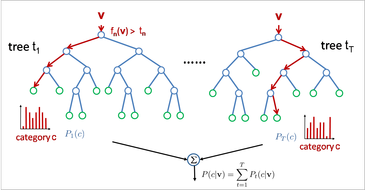
\includegraphics[width=\textwidth]{randomForestFigure.png}
    \caption{Random Forest (ensemble method).}
\end{figure}

\subsection{Neural Networks}
They are cool...

 %%% Local Variables: ***
 %%% mode:latex ***
 %%% TeX-master: "../mbc_msc_thesis"
 %%% End: ***
